\documentclass[border=4pt]{standalone}
\usepackage[T1]{fontenc}
\usepackage{helvet}
\renewcommand{\familydefault}{\sfdefault}
\usepackage{graphicx}
\usepackage{caption}
\usepackage{amsmath}
\captionsetup{font={sf,footnotesize},labelfont={sf,bf,footnotesize},justification=justified,singlelinecheck=false}
\begin{document}
\setcounter{figure}{18}
\begin{minipage}{7.20in}
\centering
\begin{figure}[htbp]
    \centering
    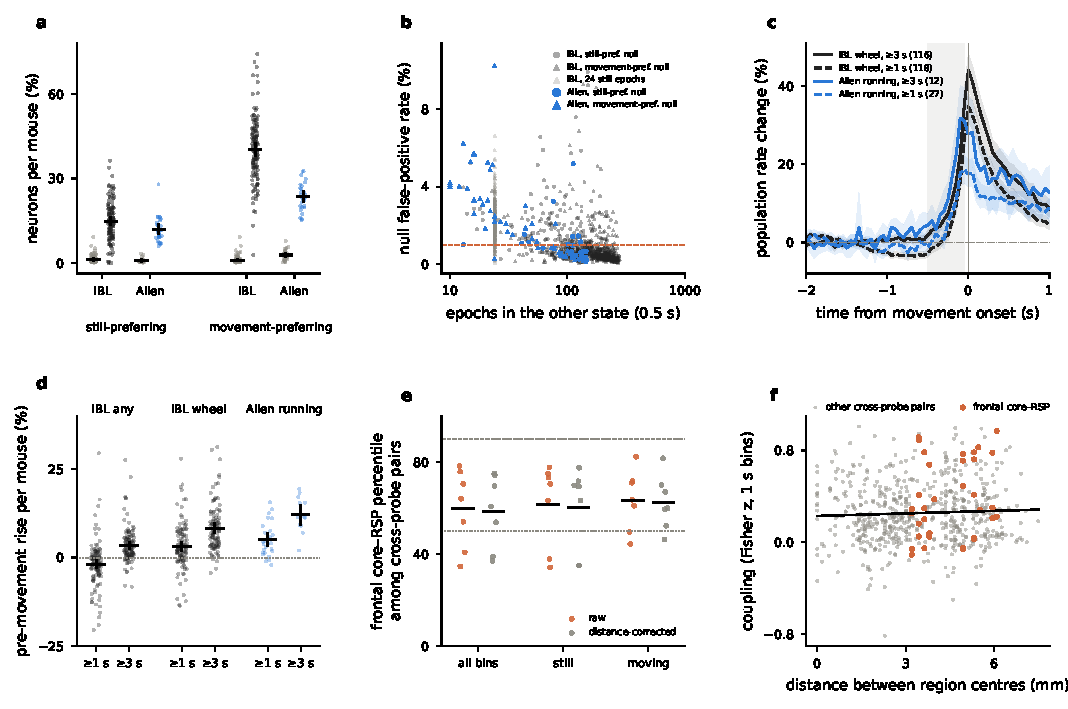
\includegraphics[width=\linewidth]{fig19_allen_followup_panels.pdf}
    \caption{Allen follow-up analyses and their IBL counterparts: label calibration, onset rule and frontal--retrosplenial coupling. \textbf{a} Still- and movement-preferring neurons per mouse (colour) against their circular-shift null (grey): all neurons' grey-screen 50\,ms counts rotated together against the fixed behavioural labels (200 offsets $\geq$10\,s per session) and the epoch test repeated. IBL: 386 sessions, 129 mice, report definition; Allen: Visual Behavior, 44 sessions, 30 mice (follow-up export). Black: mean and 95\% bootstrap CI over mice. \textbf{b} Null false-positive rate per session against the number of epochs in the opposite state. Grey triangles: IBL movement-preferring null with still epochs subsampled to 24, the Allen median. Dashed: nominal 1\%. \textbf{c} Population rate around movement onsets preceded by $\geq$3\,s (solid) or $\geq$1\,s (dashed) of awake stillness, percent change from the $-2$ to $-1$\,s mean; mean over mice (number in brackets) and 95\% bootstrap CI. IBL: wheel onsets (wheel-only states); Allen: running onsets. Shaded: $-0.5$ to $-0.05$\,s. \textbf{d} Rise ($-0.5$ to $-0.05$\,s against $-2$ to $-1$\,s) per mouse for each onset rule: IBL any-movement onsets (report definition), IBL wheel onsets and Allen running onsets; sessions with $\geq$3 onsets. \textbf{e} Allen OpenScope (8 sessions, 7 mice with a frontal core and an RSP region on different probes): percentile of each mouse's frontal core--RSP pairs among all cross-probe region pairs of the session, from Fisher $z$ of 1\,s regional rates (60\,s running mean removed), in all, still and moving bins (passive viewing; running $>$2\,cm/s; still = no running within $\pm$1\,s); raw (orange) and after removing a per-session linear fit on distance (grey). Bars: mean over mice. Dotted: 50th, dashed: 90th percentile. \textbf{f} Coupling against the distance between Allen CCF region centres for all 614 cross-probe pairs of the 11 sessions; orange, frontal core--RSP pairs; line, linear fit.}
    \label{fig:allen_followup}
\end{figure}
\end{minipage}
\end{document}
